\begin{frame}{Introduction}
We have seen already how bases can be used to help computationally understand vector spaces and their subspaces; we will now see how they can be used to analyze and understand linear transformations. 

\bspace Given a linear transformation $T\colon V\rightarrow W$, one thing we want to understand are the associated subspaces $\NS T\subseteq V$ and $\range T\subseteq W$. The \alert{rank-nullity} theorem, sometimes called the \alert{fundamental theorem of linear algebra}, relates the dimension of these two spaces with the dimension of $V$.   

\end{frame}
\begin{frame}
\begin{theorem}[Rank-nullity theorem]
Let $V$ be a vector space with $\dim V=n<\infty$. Let $T\colon V\rightarrow W$ be a linear transformation. (We make no assumption about the dimension of $W$.) Then: 
\[
\dim\NS T+\dim\range T=n.
\]
\end{theorem}
\pause
\begin{comment}
We define the {\bf nullity} of $T$ as $\nullity T=\dim\NS T$, and the {\bf rank} of $T$ as $\rank T=\dim\range T$. The rank-nullity theorem thus asserts that $\nullity T+\rank T=\dim V$. 
\end{comment}
\pause \begin{proof}[Proof of rank-nullity theorem]
Let  $B_1=\{\boldv_1,\boldv_2,\dots, \boldv_r\}$ be a basis for $\NS T$. (It is possible to find such a finite basis since $W\subseteq V$ and $\dim V=n$.)
\bpause
Extend $B_1$ to a basis $B=\{\boldv_1,\boldv_2,\dots, \boldv_r, \boldv_{r+1},\boldv_{r+2},\dots, \boldv_n\}$ of $V$. (This is possible by the dimension theorem compendium. Note that in total $B$ will have $n$ elements.) 
\bpause \alert{Claim}: $B_2=\{T(\boldv_{r+1}), T(\boldv_{r+2}), \dots, T(\boldv_{n})\}$ is a basis for $\range T\subseteq W$. 
\bpause
I will prove the claim on the next slide. Assuming the claim is true, we are done since then 
\[
n=r+(n-r)=\#B_1+\#B_2=\dim\NS T+\dim\range T.
\]
\end{proof}
\end{frame}
\begin{frame}
 \begin{proof}[Proof of claim]
 We let $B_2=\{T(\boldv_{r+1}), T(\boldv_{r+2}), \dots, T(\boldv_{n})\}$, with notation as in the previous slide. 
\bspace
\alert{$B_2$ is linearly independent}. 
\bspace If
$ c_{r+1}T(\boldv_{r+1})+c_{r+2}T(\boldv_{r+2})+ \dots+c_{n}T(\boldv_{n})=\boldzero_W$, then $T(c_r\boldv_{r}+c_{r+1}\boldv_{r+2}+ \dots+c_{n}\boldv_{n})=\boldzero_W$, since $T$ is linear. 
\bpause Then $\boldv=c_r\boldv_{r}+c_{r+1}\boldv_{r+2}+ \dots+c_{n}\boldv_{n}\in\NS T$. 
\bpause Then we can write $\boldv=c_1\boldv_1+c_2\boldv_2+\cdots +c_r\boldv_r$, since $B_1$ is a basis for $\NS T$. 
\bpause 
Then $c_1\boldv_1+c_2\boldv_2+\cdots +c_r\boldv_r=\boldv=c_r\boldv_{r}+c_{r+1}\boldv_{r+2}+ \dots+c_{n}\boldv_{n}$, and hence $c_1\boldv_1+c_2\boldv_2+\cdots +c_r\boldv_r-c_{r+1}\boldv_{r+1}- \dots-c_{n}\boldv_{n}=\boldzero$
\bpause 
Then $c_1=c_2=\dots=c_{r+1}=c_{r+2}=\cdots =c_n=0$, since $B$ is a basis. This implies the original linear combination of the $T(\boldv_i)$ was trivial, and thus that $B_2$ is independent. 
 \bpause \alert{$B_2$ spans $\range T$.}
 Take $\boldw\in \range T$. Then $w=\boldv$ for some $\boldv\in V$.
 \bpause
 Write $\boldv=c_1\boldv_1+\cdots +c_r\boldv_r+c_{r+1}\boldv_{r+1}+\cdots +c_n\boldv_n$. (Possible since $B$ is a basis.) 
 
 \pause 
 Then 
 $\boldw=T(\boldv)=T(\sum_{i=1}^nc_i\boldv_i)=\sum_{i=1}^nc_iT(\boldv_i)$, since $T$ is linear.
 \bpause 
 But we have $\sum_{i=1}^nc_iT(\boldv_i)=0+0+\cdots +0+\sum_{i=r+1}^nc_iT(\boldv_i)$, since $\boldv_i\in\NS T$ for $1\leq i\leq r$. 
 \bpause 
 Thus $\boldw=c_{r+1}T(\boldv_{r+1})+c_{r+2}T(\boldv_{r+2})+\cdots c_nT(\boldv_n)$, showing that $\boldw\in \Span B_2$, and thus that $\range T\subseteq\Span B_2$. Since clearly $\Span B_2\subseteq\range T$, we have $\Span B_2=\range T_2$, as desired. 
 \end{proof}
\end{frame}
\begin{frame}
 \begin{example}
 Let $T=T_A$ where 
 \[
 A=\begin{bmatrix}
 1&0&-1&2\\
 2&1&1&1
 \end{bmatrix}
 \]
 A little Gaussian elimination shows that $\NS A=\{(s-2t,-3(s-t),s,t)\colon s, t\in\R\}$. 
 \bpause
 Notice that the general form of an element of $\NS A$ can be expressed as 
 \[
 (s-2t,-3(s-t),s,t)=s(1,-3,1,0)+t(-2,3,0,1).
 \]
 From this it follows that $B=\{ (1,-3,1,0), (-2,3,0,1)\}$ is a basis for $\NS A$, and thus that $\dim\NS A=2$.
 \bpause
 The rank-nullity theorem now implies that $\dim \range T=\dim \R^4-\dim\NS A=4-2=2$. Since $\range T\subseteq\R^2$ and $\dim\range T=2$, we conclude from the dimension theorem compendium that $\range T=\R^2$. 
 \bpause
 Thanks to the rank-nullity theorem, our quick computation of $\NS A$ allowed us to determine $\range T$ with minimal additional effort! 
 \end{example}
\end{frame}
\begin{frame}
 \begin{example}
 Let $T\colon \R^3\rightarrow \R^3$ be orthogonal projection onto the plane $W: x+y+z=0$, as defined earlier. 
 \bspace
 It is clear that $\range T=W$. Indeed $T$ maps all vectors to vectors in $W$, by definition, so $\range T\subseteq W$. Furthermore, given any $\boldw\in W$, we have $\boldw=T(\boldw)$, since orthogonal projection does nothing to a vector that already lies in $W$. 
This proves $\range T=W$. It follows that $\rank T=\dim W=2$. 
  \bpause
  The rank-nullity theorem then implies $\dim \NS T=3-2=1$. So $\NS T$ is a line (dimension-1 subspace) passing through the origin. Which one? Geometrically this is easy to see: it is $\Span(\{(1,1,1)\})$, the line passing through the origin and orthogonal to $W$. 
 \[
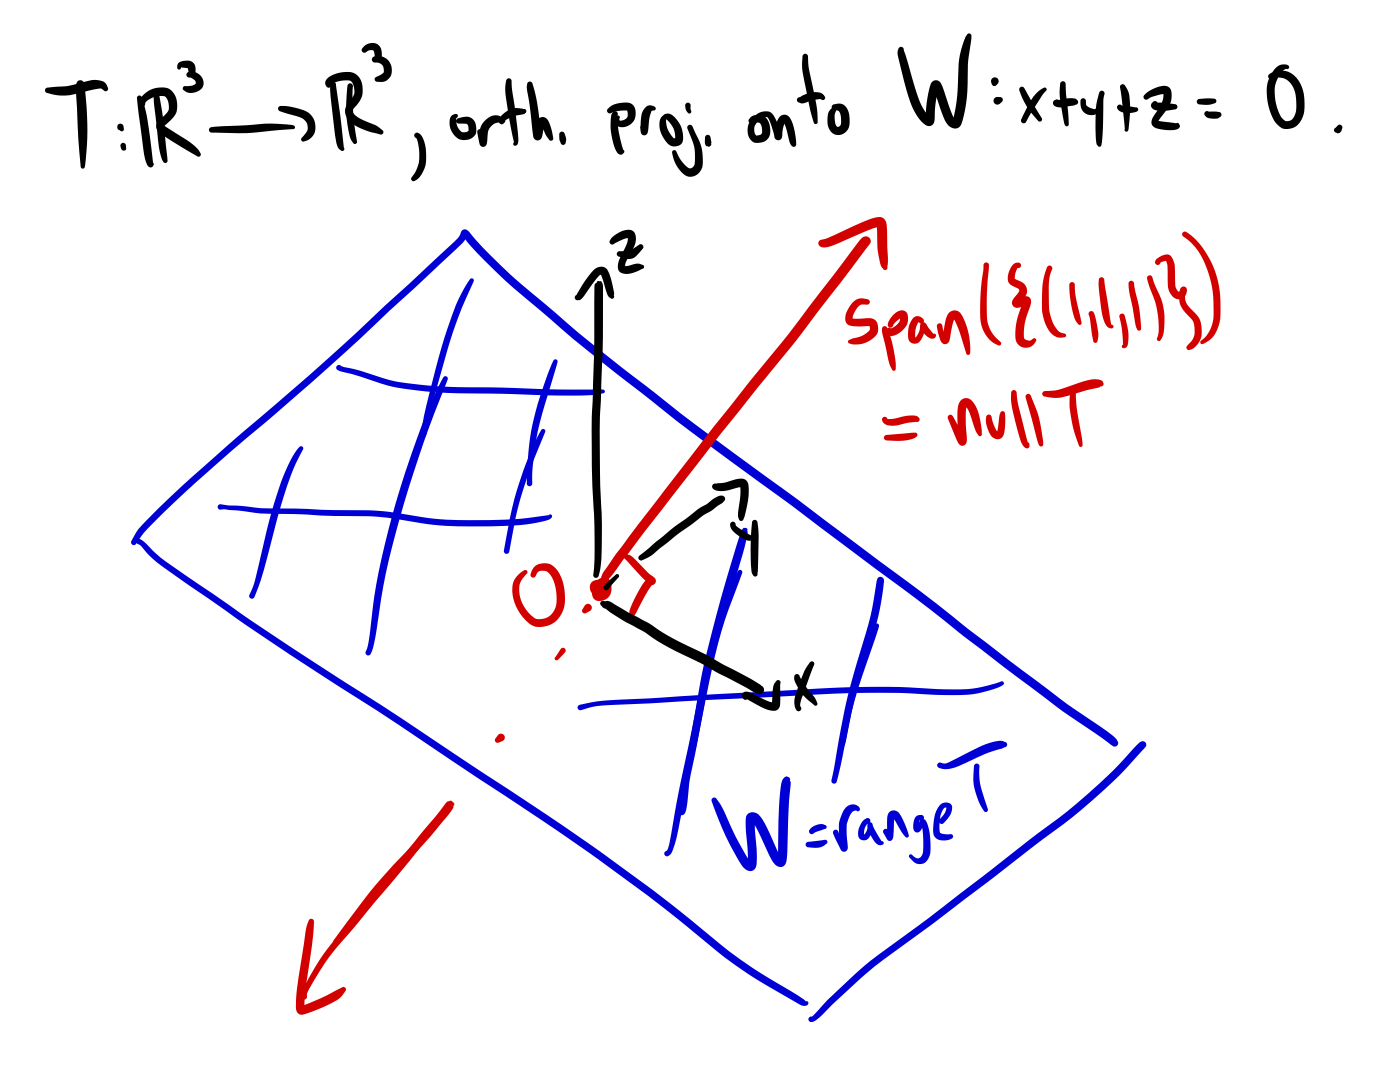
\includegraphics[width=2.5in]{Images/OrthoRankNull}
\]
  \end{example}
\end{frame}
\begin{frame}
 \begin{example}
 Define $T\colon M_{nn}\rightarrow M_{nn}$ as $T(A)=A^T-A$. 
 \bspace 
 As we have seen elsewhere, $\NS T=\{A\in M_{nn}\colon A^T=A\}$ and $\range T=\{A\in M_{nn}\colon A^T=-A\}$, the space of symmetric and skew-symmetric matrices, respectively.  
 \bpause 
 As we have also seen, the dimension of the space of symmetric matrices is $\frac{n(n+1)}{2}$, and the dimension of skew-symmetric matrices is $\frac{n(n-1)}{2}$. 
 \bspace
 According to the rank-nullity theorem we must have 
 \begin{align*}
 n^2&=M_{nn}\\
 &=\dim\NS T+\dim\range T\\
 &=\frac{n(n+1)}{2}+\frac{n(n-1)}{2}.
 \end{align*}
 We have thus given a linear algebraic proof of the identity $n^2=\frac{n(n+1)}{2}+\frac{n(n-1)}{2}$. 
 \bpause
 Yes, there is a more straightforward arithmetic proof, but you must admit this one is pretty cool, and it illustrates how results in one area of mathematics (e.g., linear algebra) can sometimes be translated into results in a completely different area (e.g., combinatorics). 
 
 \end{example}
\end{frame}
\begin{frame}{Relative sizes of $\NS T$ and $\range T$}
Let $T\colon V\rightarrow W$, where $\dim V=n$. Since 
$
\dim\NS T+\dim\range T=n,
$
we see that the {\color{red} bigger} the null space (dimension-wise), the {\color{blue} smaller} the range, and vice versa. 

Let's see this numerically in action. Assume $T\colon V\rightarrow W$ is linear. 
\bb
\pause\ii Suppose $\dim V=5$ and $\dim W=3$. Prove: $\NS T$ is nontrivial. 
\bpause
If $\NS T=\{\boldzero\}$, then $\dim\range T=5-0=5$; but this is impossible since $\range T\subseteq W$ and $\dim W=3$. Thus $\NS T\ne \{\boldzero\}$; i.e., there is a nonzero $\boldv\in\NS T$. This shows $\NS T$ is nontrivial. 
\pause\ii Suppose $\dim V=7$, $\dim W=5$, and $\dim\NS T=2$. Prove: $\range T= W$. 
\bpause 
We have $\dim\range T=7-\dim\NS T=7-2=5$. Since $\range T\subseteq W$ and $\dim\range T=\dim W$, we conclude $\range T=W$. 
\ee
\end{frame}

\begin{frame}{Fundamental subspaces of a matrix}
When $T=T_A$ for some $m\times n$ matrix $A$, we can develop a systematic way of computing bases for $\NS A$ and $\range A$. Not surprisingly this procedure involves Gaussian elimination, as we will outline below. 
\bspace 
In fact the procedure allows us to compute bases for the three following subspaces associated to a matrix, the so-called \alert{fundamental subspaces} of $A$. 

\pause
\begin{definition}
Let $A$ be a an $m\times n$ matrix with rows $\boldr_1,\dots, \boldr_m$ and columns $\boldc_1,\dots \boldc_n$. The following subspaces are called the {\bf fundamental subspaces of $A$}. 
\bb
\ii The {\bf null space} of $A$ is defined as 
\[
\NS A =\{\boldx\in\R^n\colon A\boldx=\boldzero\}\subset \R^n.
\]
\ii The {\bf row space} of $A$ is defined as 
\[
\RS A =\Span(\{\boldr_1,\dots, \boldr_m\})\subset\R^n.
\]
\ii The {\bf column space} of $A$ is defined as 
\[
\CS A=\Span(\{\boldc_1,\dots \boldc_n\})\subset\R^m. 
\]
\ee
\end{definition}
\pause 
The careful reader will object that $\range A$ does not appear on this list! Fear not, as we show in the next slide \alert{$\CS A=\range A$}. 
\end{frame}

\begin{frame}{$\CS A=\range A$}
Take an $m\times n$ matrix and consider $A$ as a collection of $n$ columns $\boldc_j$, each of which lives in $\R^m$:
\[
A=\begin{bmatrix}
\vert&\vert& \cdots &\vert\\
\boldc_1&\boldc_2&\cdots &\boldc_n\\
\vert&\vert& \cdots &\vert
\end{bmatrix}
\]
\pause
Then we have 
\begin{eqnarray*}
\boldb\in\CS A &\Leftrightarrow& \boldb\in\Span(\{\boldc_1,\dots,\boldc_n\})\\
\pause&\Leftrightarrow & \boldb=a_1\boldc_1+a_2\boldc_2+\cdots + a_n\boldc_n \text{ for some $a_i$}\\
\pause&\Leftrightarrow & \boldb=A\begin{bmatrix}
a_1\\ a_2\\ \vdots \\ a_n
\end{bmatrix} \text{ (by column expansion!!)} \\
\pause&\Leftrightarrow & \text{ there is an $\boldx\in\R^n$ such that } A\boldx=\boldb \\
\pause&\Leftrightarrow &\boldb\in \range A.
\end{eqnarray*}
We conclude:
\[
\boxed{\CS A=\range A}
\]
\end{frame}

\begin{frame}{Computing the fundamental spaces}
\footnotesize
Once again Gaussian elimination is the main tool for computing fundamental spaces: start with $A$, row reduce to $U$, compute the fundamental spaces of $U$. However, there are some subtleties involved. Here is the overall description for how to proceed:
\[
\pause 
\begin{array}{lcl}
\text{Space}&\text{Relation}&\text{How to pick a basis}\\
\hline
\text{Null space}&\NS A=\NS U&\left(\begin{array}{c}\text{find vector parametrization}\\ \text{of solutions to $U\boldx=\boldzero$} \end{array}\right) \\
\\
\pause\text{Row space}&\RS A=\RS U &\left(\begin{array}{c}\text{nonzero rows of $U$ }\\ \text{form a basis of $\RS(A)$} \end{array}\right) \\
\\
\pause\text{Column space}&\CS A \alert{\ne}\CS U &\left(\begin{array}{c}\text{pick columns of $A$ corresponding}\\ \text{to columns of $U$ with leading 1's} \end{array}\right) 
\end{array}
\]
\end{frame}
\begin{frame}
Let's prove some of the previous claims. We will begin by proving the following more general result.
\bspace
\alert{Claim}. If $A$ and $B$ are \alert{row equivalent}, then $\NS(A)=\NS(B)$, $\RS(A)=\RS(B)$, and if a certain subset of the columns of $B$ form a basis of $\CS(B)$, then the same is true of the corresponding columns of $A$ and $\CS(A)$. 
\pause
\begin{proof}
First observe that $A$ is row equivalent to $B$ iff $(E_rE_{r-1}\cdots E_1)A=B$ for some elementary matrices $E_i$ iff $QA=B$ for some invertible $Q$. (The latter ``iff" follows since the $E_i$ are elementary, and since all invertible matrices are products of elementary matrices. )
\pause
So we assume $QA=B$ for some invertible $Q$. 
\bpause 
\alert{Null space}. We have shown in an exercise that $A\boldx=\boldzero$ iff $QA\boldx=\boldzero$ iff $B\boldx=\boldzero$. It follows that $\NS(A)=\NS(B)$. 
\bpause
\alert{Row space}
To show $\RS(A)=\RS(B)$, it is enough to show that $\RS(B)\subseteq \RS(A)$; this is because we can then apply the same reasoning using the fact that $A=Q^{-1}B$, $Q^{-1}$ invertible. \pause The row method tells us that each row of $B=QA$ is a linear combination of the rows of $A$. Thus each row of $B$ lies in $\RS(A)$, the span of the rows of $A$. \pause But then we must have $\RS(B)\subseteq\RS(A)$, since $\RS(B)$ is the ``smallest" subspace containing all rows of $B$ (by properties of span).
\bpause
\alert{Column space} (Sketch). Here one can show that columns $\boldc_{i_1}, \boldc_{i_2},\dots, \boldc_{i_r}$ of $A$ form a basis of $\CS(A)$ iff $Q\boldc_{i_1}, Q\boldc_{i_2},\dots, Q\boldc_{i_r}$ form a basis of $\CS(B)$. By the column method the vectors $Q\boldc_{i_j}$ are precisely the corresponding columns of $B=QA$. 
\end{proof}

\end{frame}
\begin{frame}{Example}
\footnotesize
Let's compute bases/dimensions for the fundamental spaces of \\ 
$A=\begin{bmatrix}[rrrr]
2&2&4&2\\
6&6&11&5\\
-4&-4&-7&-3
\end{bmatrix}
$.\\
\pause $A$ reduces to the matrix 
$U=\begin{bmatrix}[rrrr]
1&1&2&1\\
0&0&1&1\\
0&0&0&0
\end{bmatrix}
$
\bpause
First compute 
\[
\NS(U)=\{(s-r,r,-s,s)\colon r, s\in\R\}=\{s(1,0,-1,1)+r(-1,1,0,0)\colon r,s\in\R\}.
\]
It follows that $\NS A=\NS U=\Span \{(1,0,-1,1), (-1,1,0,0)\}$, and thus that $B=\{(-1,1,0,0), (1,0,-1,1)\}$ is a basis for $\NS(A)$. We conclude $\dim\NS A=2$. 
\bpause Next, the rank-nullity theorem implies $\dim\range U=\dim \R^4-\dim\NS U=2$. Thus to choose a basis for $\CS U=\range U$ we need only pick two linearly independent columns of $U$:  the first and third columns will do. It follows that the first and third columns of $A$ form a basis for $\CS A$. This gives us $B''=\{(2,6,-4), (4,11,-7)\}$ as a basis for $\CS A $. 
\bpause
Finally, we have $\RS A =\RS U$, and clearly we can take the nonzero rows of $U$ as a basis for this. Thus $B'=\{(1,1,2,1),(0,0,1,1)\}$ is a basis for $\RS A $. We conclude $\dim\RS A=2$. 
\end{frame}
\begin{frame}
 The preceding example nicely illustrates our general procedure for computing bases for the fundamental spaces of $A$. 
 \begin{block}{Computing bases for the fundamental spaces}
\bb[(i)]
\ii Reduce $A$ to row echelon form matrix $U$. 
\ii $\boxed{\NS(A)=\NS(U)}$. Use free/leading variable method to give full description of solutions $U\boldx=\boldzero$. Extract a basis from the resulting parametric description. 
\ii $\boxed{\RS(A)=\RS(U)}$. A basis for $\RS(U)$ (and hence $\RS(A)$) consists of the nonzero rows of $U$. 
\ii $\boxed{\CS(A)\ne \CS(U)}$. The columns of $U$ with leading 1's are a basis for $\CS(U)$. The {\em corresponding columns} of $A$ form a basis for $\CS(A)$. 
\ee
\end{block}
\pause
\begin{comment}
It is clear that the nonzero rows of $U$ form a basis of $\RS U$: the staircase pattern of leading 1's guarantees they are linearly independent, and we can obviously discard the zero rows. 
\bpause
It is not difficult to show that the columns of $U$ with leading 1's are linearly independent. (Exercise!) That they are in fact a basis follows from the fact that $\#\text{(leading 1's)}=n-\#\text{(free variables)}=n-\dim\NS U=\dim\CS U$. 
\end{comment}
\end{frame}
\begin{frame}{Rank-nullity theorem for matrices}
The previous discussion gives us a much more detailed analysis of the spaces involved in the rank-nullity theorem in the special case where $T=T_A$. We collect some of those details here. 
\begin{block}{Rank-nullity theorem for matrices}
Let $A$ be $m\times n$. Suppose $A$ is row equivalent to the row echelon matrix $U$. 
\bb
\ii $\CS A=\range A$
\ii $\dim\NS A=\#(\text{free variables in the system $U\boldx=\boldzero$})$
\ii $\rank A=\dim\CS A=\dim\RS A=\#(\text{leading 1's in $U$})$
\ii $\rank A\leq \min\{m,n\}$. (Since $\#(\text{leading 1's in $U$})\leq m$ and $\#(\text{leading 1's in $U$})\leq n$.) 
\ii $n=\dim\NS A+\dim\CS A=\dim\NS A+\dim\RS A$. 
\ee
\end{block}
\end{frame}
\begin{frame}{Extending/contracting sets to bases}
Recall that if $\dim V=n$, then any linearly independent set can be \alert{extended} to a basis of $B$, and any spanning set can be \alert{contracted} to a basis. 

In the special case when $V=\R^n$, our fundamental space algorithms provide a means of performing these extensions/contractions. \bpause
Let $\boldv_1,\boldv_2, \dots, \boldv_r\in \R^n$. 
\bb
\ii \alert{Extending to basis}. If the $\boldv_i$ are independent, then to extend to a basis of $\R^n$ proceed as follows:
\bb
\ii Build the matrix $A$ whose columns (in order) are $\boldv_1,\boldv_2, \dots, \boldv_r, \bolde_1,\bolde_2,\dots, \bolde_n$.
\ii Apply the column space algorithm to $A$. 
\ee
\ii \alert{Contracting to basis}. If the $\boldv_i$ span the subspace$W\subseteq\R^n$, then to contract to a basis of $W$ proceed as follows:
\bb
\ii Build the matrix $A$ whose columns are $\boldv_1, \boldv_2, \dots, \boldv_r$. 
\ii Apply the column space algorithm to $A$. 
\ee


\ee
\end{frame}
\begin{frame}{Example}
\footnotesize
Let $W=\Span\{\boldv_1,\boldv_2, \boldv_3, \boldv_4, \boldv_5\}$ where 
\[
\begin{array}{ll}
\boldv_1=(1,-1,5,2)&\boldv_2=(-2,3,1,0)\\
\boldv_3=(4,-5,9,4)&\boldv_4=(0,4,2,-3)\\
\boldv_5=(-7,18,2,-8)
\end{array}
\]
Find a subset of the $\boldv_i$ that yields a basis of $W$. 
\bpause 
We know the $\boldv_i$ span $W$, so to get a basis we need to ``throw out the redundant ones". To figure out which ones need to go, we create a matrix $A$ by setting the $\boldv_i$ as  its \alert{columns} (not its rows)! The procedure for finding a basis for $\CS(A)$ then gives us a subset of these columns that forms a basis.
\bpause 
$A=\begin{bmatrix}[rrrrr]
1&-2&4&0&-7\\
-1&3&-5&4&18\\
5&1&9&2&2\\ 
2&0&4&-3&-8
\end{bmatrix}
\xrightarrow[]{\text{row red.}}
U=
\begin{bmatrix}[rrrrr]
\boxed{1}&0&2&0&-1\\
0&\boxed{1}&-1&0&3\\
0&0&0&\boxed{1}&2\\
0&0&0&0&0
\end{bmatrix}
$
\bpause
It follows that $\{\boldv_1,\boldv_2, \boldv_4\}$ is a basis for $W$. 
\end{frame}
\begin{frame}{Example}
Extend the set $S=\{ (1,1,1,1), (-2,-2,3,3)\}$ to a basis of $\R^4$. 
\bpause
Take the matrix 
\[
A=\begin{bmatrix}
1&-2&1&0&0&0\\
1&-2&0&1&0&0\\
1&3&0&0&1&0\\
1&3&0&0&0&1
\end{bmatrix}
\]
This matrix row reduces to 
\[
U=\begin{bmatrix}
\boxed{1}&-2&1&0&0&0\\
0&\boxed{1}&-1/5&0&1/5&0\\
0&0&\boxed{1}&-1&0&0\\
0&0&0&0&\boxed{1}&-1
\end{bmatrix}
\]
\pause
It follows that the first, second, third and fifth column of $A$ form a basis of $\CS(A)=\R^4$. Thus 
\[
B=\{(1,1,1,1), (-2,-2,3,3), (1,0,0,0), (0,0,1,0)\}
\]
is a basis of $\R^4$ extending $S$. 

\end{frame}
%\begin{frame}{Working in other spaces $V$}
%These algorithms gives us means of computing bases for subspaces inside $\R^n$. What about more exotic vector spaces, like $P_n$, $M_{mn}$, etc.? 
%\bspace 
%The trick when working in one of these more abstract spaces is to first pick a basis $B$ of $V$ (oftentimes the ``standard" one), and use the coordinate vector operator 
%\[
%\boldv\mapsto [\boldv]_B\in\R^n
%\]
%to translate the problem into a question about vectors in $\R^n$. 
%\bpause Use one of the previous algorithms to solve the corresponding problem in $\R^n$, then translate your results back in terms of the original vector space $V$. 
%\bspace The following examples illustrate this technique. 
%\end{frame}
%\begin{frame}{Example}
%Let $W=\Span\{p_1,p_2, p_3, p_4, p_5\}\subset P_3$ where 
%\[
%\begin{array}{ll}
%p_1=1-x+5x^2+2x^3&p_2=-2+3x+x^2\\
%p_3=4-5x+9x^2+4x^3&p_4=4x+2x^2-3x^3\\
%p_5=-7+18x+2x^2-8x^3
%\end{array}
%\]
%Find a subset of the $p_i$ that yields a basis of $W$. 
%\bpause 
%Let $B=\{1,x,x^2, x^3\}$ be the standard basis for $P_3$. Apply $[\hspace{10pt}]_B$ to each of the $p_i$ to get the exact same vectors $\boldv_i$ from the previous example.
%\bpause As we saw in that example, our column space algorithm showed that $\boldv_1, \boldv_2$ and $\boldv_4$ formed a basis for the span of the $\boldv_i$. 
%\bpause 
%It follows that $\{p_1, p_2, p_4\}$ is a basis for $W$ inside $P_3$.
% 
%\end{frame}
%\begin{frame}{Example}
%Let $A_1=\begin{bmatrix}[rr]
%1&1\\-2&0
%\end{bmatrix}
%$,
%$A_2=\begin{bmatrix}[rr]
%1&-1\\-1&1
%\end{bmatrix}
%$,
%$A_3=\begin{bmatrix}[rr]
%1&1\\1&-3
%\end{bmatrix}
%$, and let $W=\Span(\{A_1,A_2,A_3\})$. 
%
%Decide whether $A=\begin{bmatrix}
%1&0\\-1&0
%\end{bmatrix}
%$
%is in $W$. 
%\bpause
%Let $B$ be the standard basis of $M_{22}$. Translate everything to $\R^4$ using $(\underline{\hspace{.2cm}})_B$. 
%\bspace We are then asking whether $\boldv=(1,0,1,0)$ is in the span of $\boldv_1=(1,1,-2,0)$, $\boldv_2=(1,-1,-1,1)$, $\boldv_3=(1,1,1,-3)$. This is equivalent to whether the matrix equation 
%\[
%\begin{bmatrix}[rrr]
%1&1&1\\
%1&-1&1\\
%-2&-1&1\\
%0&1&-3
%\end{bmatrix}
%\boldx
%=\begin{bmatrix}[r]
%1\\ 0\\-1 \\0 
%\end{bmatrix}
%\] 
%has a solution. 
%
%GE shows that in fact we can solve this. (Do it!) This means $\boldv$ is a linear combination of the $\boldv_i$, and thus that $A$ is a linear combination of the $A_i$. 
%
%We conclude $A\in W$. 
%\end{frame}


%\begin{corollary}[Corollary of R-N]
%Let $A$ be $m\times n$. 
%\bb[(i)]
%\pause\ii If $m>n$, then there is a $\boldb\in\R^m$ such that $A\boldx=\boldb$ has no solution (i.e., is inconsistent). 
%\ii If $m<n$, then there is a nontrivial $\boldx\ne\boldzero_n\in\R^n$ such that $A\boldx=\boldzero_m$. 
%\ee
%\pause
%\begin{proof}
%\ \\
%(i) If $m>n$, then $\dim(\CS(A))=\dim(\RS(A))\leq n<m$. Thus $\CS(A)\ne\R^m$, which means there is a $\boldb$ such that $A\boldx=\boldb$ has no solution. 
%\bpause
%(ii) If $m<n$, then $\dim(\CS(A))\leq m<n$. By the R-N theorem we have 
%\[
%\dim(\NS(A))=n-\dim(\CS(A))>n-n=0.
%\]
%Thus $\NS(A)$ is a nontrivial space, which means there is a $\boldx\ne\boldzero_n$ with $A\boldx=\boldzero_m$. 
%\end{proof}
%\end{corollary}
%\end{frame}
\begin{frame}{Invertibility Theorem}
\alert{Suppose $A$ is a square $n\times n$ matrix} . Recall that $A$ is invertible if and only if $A\boldx=\boldzero$ has a unique solution. This is equivalent to $\NS(A)=\{\boldzero\}$. Thus we have: 
\[
A \text{ invertible } \Leftrightarrow \NS(A)=\{\boldzero\}\Leftrightarrow \nullity(A)=0.
\]
\pause Similarly, we have $A$ invertible if and only if $A\boldx=\boldb$ has a solution \alert{for all} $\boldb\in\R^n$. As we saw earlier, $\CS(A)=\{\boldb\in\R^n\colon A\boldx=\boldb \text{ has a solution}\}$. Thus we see that 
\[
A \text{ invertible}\Leftrightarrow \CS(A)=\R^n \Leftrightarrow \rank(A)=n \Leftrightarrow \RS(A)=\R^n,
\]
where the last equivalence follows since $\RS(A)\subset\R^n$ and $\dim(\RS(A))=n$. 
\bpause 
Looks like we have quite a few new statements to add to our Invertibility Theorem! 
\end{frame}
\begin{frame}
\begin{theorem}[Invertibility theorem]
Let $A$ be $n\times n$. The following statements are equivalent. 
\bb[(a)]
\ii $A$ is invertible.
\ii $A\boldx=\boldzero$ has a unique solution (the trivial one). 
\ii $A$ is row equivalent to $I_n$, the $n\times n$ identity matrix.
\ii $A$ is a product of elementary matrices. 	
\ii $A\boldx=\boldb$ has a solution for every $n\times 1$ column vector $\boldb$. 
\ii $A\boldx=\boldb$ has a {\em unique} solution for every $n\times 1$ column vector $\boldb$. 
\ii $\det A\ne 0$.
\ii $\NS A=\{\boldzero\}$.
\ii $\nullity A=0$.
\ii $\rank A=n$. 
\ii $\CS A=\R^n$.
\ii $\RS A=\R^n$.
\ii The columns of $A$ are linearly independent (or span $\R^n$, or are a basis of $\R^n$).
\ii The rows of $A$ are linearly independent (or span $\R^n$, or are a basis of $\R^n$). 
\ee
\end{theorem}

\end{frame}






